\documentclass[11pt,a4paper]{article}
\usepackage{lmodern}

\usepackage{amssymb,amsmath}
\usepackage{ifxetex,ifluatex}
\usepackage{fixltx2e} % provides \textsubscript
\ifnum 0\ifxetex 1\fi\ifluatex 1\fi=0 % if pdftex
  \usepackage[T1]{fontenc}
  \usepackage[utf8]{inputenc}
\else % if luatex or xelatex
  \ifxetex
    \usepackage{mathspec}
    \usepackage{xltxtra,xunicode}
  \else
    \usepackage{fontspec}
  \fi
  \defaultfontfeatures{Mapping=tex-text,Scale=MatchLowercase}
  \newcommand{\euro}{€}
\fi
% use upquote if available, for straight quotes in verbatim environments
\IfFileExists{upquote.sty}{\usepackage{upquote}}{}
% use microtype if available
\IfFileExists{microtype.sty}{%
\usepackage{microtype}
\UseMicrotypeSet[protrusion]{basicmath} % disable protrusion for tt fonts
}{}
\usepackage[lmargin=5cm,rmargin=2.5cm,tmargin=2.5cm,bmargin=2.5cm]{geometry}

% Figure Placement:
\usepackage{float}
\let\origfigure\figure
\let\endorigfigure\endfigure
\renewenvironment{figure}[1][2] {
    \expandafter\origfigure\expandafter[H]
} {
    \endorigfigure
}

%% citation setup

\usepackage{csquotes}

\usepackage[backend=biber, maxbibnames = 99, style = apa]{biblatex}
\setlength\bibitemsep{1.5\itemsep}
\bibliography{references.bib}
\usepackage{color}
\usepackage{fancyvrb}
\newcommand{\VerbBar}{|}
\newcommand{\VERB}{\Verb[commandchars=\\\{\}]}
\DefineVerbatimEnvironment{Highlighting}{Verbatim}{commandchars=\\\{\}}
% Add ',fontsize=\small' for more characters per line
\usepackage{framed}
\definecolor{shadecolor}{RGB}{248,248,248}
\newenvironment{Shaded}{\begin{snugshade}}{\end{snugshade}}
\newcommand{\AlertTok}[1]{\textcolor[rgb]{0.94,0.16,0.16}{#1}}
\newcommand{\AnnotationTok}[1]{\textcolor[rgb]{0.56,0.35,0.01}{\textbf{\textit{#1}}}}
\newcommand{\AttributeTok}[1]{\textcolor[rgb]{0.77,0.63,0.00}{#1}}
\newcommand{\BaseNTok}[1]{\textcolor[rgb]{0.00,0.00,0.81}{#1}}
\newcommand{\BuiltInTok}[1]{#1}
\newcommand{\CharTok}[1]{\textcolor[rgb]{0.31,0.60,0.02}{#1}}
\newcommand{\CommentTok}[1]{\textcolor[rgb]{0.56,0.35,0.01}{\textit{#1}}}
\newcommand{\CommentVarTok}[1]{\textcolor[rgb]{0.56,0.35,0.01}{\textbf{\textit{#1}}}}
\newcommand{\ConstantTok}[1]{\textcolor[rgb]{0.00,0.00,0.00}{#1}}
\newcommand{\ControlFlowTok}[1]{\textcolor[rgb]{0.13,0.29,0.53}{\textbf{#1}}}
\newcommand{\DataTypeTok}[1]{\textcolor[rgb]{0.13,0.29,0.53}{#1}}
\newcommand{\DecValTok}[1]{\textcolor[rgb]{0.00,0.00,0.81}{#1}}
\newcommand{\DocumentationTok}[1]{\textcolor[rgb]{0.56,0.35,0.01}{\textbf{\textit{#1}}}}
\newcommand{\ErrorTok}[1]{\textcolor[rgb]{0.64,0.00,0.00}{\textbf{#1}}}
\newcommand{\ExtensionTok}[1]{#1}
\newcommand{\FloatTok}[1]{\textcolor[rgb]{0.00,0.00,0.81}{#1}}
\newcommand{\FunctionTok}[1]{\textcolor[rgb]{0.00,0.00,0.00}{#1}}
\newcommand{\ImportTok}[1]{#1}
\newcommand{\InformationTok}[1]{\textcolor[rgb]{0.56,0.35,0.01}{\textbf{\textit{#1}}}}
\newcommand{\KeywordTok}[1]{\textcolor[rgb]{0.13,0.29,0.53}{\textbf{#1}}}
\newcommand{\NormalTok}[1]{#1}
\newcommand{\OperatorTok}[1]{\textcolor[rgb]{0.81,0.36,0.00}{\textbf{#1}}}
\newcommand{\OtherTok}[1]{\textcolor[rgb]{0.56,0.35,0.01}{#1}}
\newcommand{\PreprocessorTok}[1]{\textcolor[rgb]{0.56,0.35,0.01}{\textit{#1}}}
\newcommand{\RegionMarkerTok}[1]{#1}
\newcommand{\SpecialCharTok}[1]{\textcolor[rgb]{0.00,0.00,0.00}{#1}}
\newcommand{\SpecialStringTok}[1]{\textcolor[rgb]{0.31,0.60,0.02}{#1}}
\newcommand{\StringTok}[1]{\textcolor[rgb]{0.31,0.60,0.02}{#1}}
\newcommand{\VariableTok}[1]{\textcolor[rgb]{0.00,0.00,0.00}{#1}}
\newcommand{\VerbatimStringTok}[1]{\textcolor[rgb]{0.31,0.60,0.02}{#1}}
\newcommand{\WarningTok}[1]{\textcolor[rgb]{0.56,0.35,0.01}{\textbf{\textit{#1}}}}
\usepackage{graphicx}
\makeatletter
\def\maxwidth{\ifdim\Gin@nat@width>\linewidth\linewidth\else\Gin@nat@width\fi}
\def\maxheight{\ifdim\Gin@nat@height>\textheight\textheight\else\Gin@nat@height\fi}
\makeatother
% Scale images if necessary, so that they will not overflow the page
% margins by default, and it is still possible to overwrite the defaults
% using explicit options in \includegraphics[width, height, ...]{}
\setkeys{Gin}{width=\maxwidth,height=\maxheight,keepaspectratio}
\ifxetex
  \usepackage[setpagesize=false, % page size defined by xetex
              unicode=false, % unicode breaks when used with xetex
              xetex]{hyperref}
\else
  \usepackage[unicode=true]{hyperref}
\fi
\hypersetup{breaklinks=true,
            bookmarks=true,
            pdfauthor={Name},
            pdftitle={Title},
            colorlinks=true,
            citecolor=blue,
            urlcolor=blue,
            linkcolor=magenta,
            pdfborder={0 0 0}}
\urlstyle{same}  % don't use monospace font for urls
\setlength{\parindent}{0pt}
\setlength{\parskip}{6pt plus 2pt minus 1pt}
\setlength{\emergencystretch}{3em}  % prevent overfull lines
\setcounter{secnumdepth}{5}

%%% Use protect on footnotes to avoid problems with footnotes in titles
\let\rmarkdownfootnote\footnote%
\def\footnote{\protect\rmarkdownfootnote}

%%% Change title format to be more compact
\usepackage{titling}

% Create subtitle command for use in maketitle
\newcommand{\subtitle}[1]{
  \posttitle{
    \begin{center}\large#1\end{center}
    }
}

\setlength{\droptitle}{-2em}
  \title{Title}
  \pretitle{\vspace{\droptitle}\centering\huge}
  \posttitle{\par}
\subtitle{Subtitle}
  \author{Name}
  \preauthor{\centering\large\emph}
  \postauthor{\par}
  \predate{\centering\large\emph}
  \postdate{\par}
  \date{today}


%% linespread settings

\usepackage{setspace}

\onehalfspacing

% Language Setup

\usepackage{ifthen}
\usepackage{iflang}
\usepackage[super]{nth}
\usepackage[ngerman, english]{babel}

\begin{document}

\selectlanguage{english}


%\maketitle

\newgeometry{left=2cm,right=1cm,bottom=2cm,top=2cm}

\begin{titlepage}
  \noindent\begin{minipage}{0.6\textwidth}
	  \IfLanguageName{english}{University of Duisburg-Essen}{Universität Duisburg-Essen}\\
	  \IfLanguageName{english}{Faculty of Business Administration and Economics}{Fakultät für Wirtschaftswissensschaften}\\
	  \IfLanguageName{english}{Chair of Econometrics}{Lehrstuhl für Ökonometrie}\\
  \end{minipage}
	\begin{minipage}{0.4\textwidth}
	  \begin{flushright}
  	  \vspace{-0.5cm}
      \IfLanguageName{english}{\includegraphics*[width=5cm]{Includes/duelogo_en.png}}{\includegraphics*[width=5cm]{Includes/duelogo_de.png}}
	  \end{flushright}
	\end{minipage}
  \\
  \vspace{1.5cm}
  \begin{center}
  \huge{Title}\\
  \vspace{.25cm}
  \Large{Subtitle}\\
  \vspace{0.5cm}
  \large{Type of Paper}\\
  \vspace{1cm}
  \large{
  \IfLanguageName{english}{Submitted to the Faculty of \\ Business Administration and Economics \\at the \\University of Duisburg-Essen}{Vorgelegt der \\Fakultät für Wirtschaftswissenschaften der \\ Universität Duisburg-Essen}\\}
  \vspace{0.75cm}
  \large{\IfLanguageName{english}{from:}{von:}}\\
  \vspace{0.5cm}
  Name\\
  \end{center}
  \vspace{4cm}

  \noindent\begin{minipage}[t]{0.5\textwidth}
  \IfLanguageName{english}{Matriculation Number:}{Matrikelnummer}
  \end{minipage}
  \begin{minipage}[t]{0.7\textwidth}
  \hspace{1cm}Matriculation Number
  \end{minipage}

  \noindent\begin{minipage}[t]{0.5\textwidth}
  \IfLanguageName{english}{Study Path:}{Studienfach:}
  \end{minipage}
  \begin{minipage}[t]{0.7\textwidth}
  \hspace{1cm}Study Path
  \end{minipage}

  \noindent\begin{minipage}[t]{0.5\textwidth}
  \IfLanguageName{english}{Reviewer:}{Erstgutachter:}
  \end{minipage}
  \begin{minipage}[t]{0.7\textwidth}
  \hspace{1cm}Prof.~Dr.~Christoph Hanck
  \end{minipage}

  \noindent\begin{minipage}[t]{0.5\textwidth}
  \IfLanguageName{english}{Secondary Reviewer:}{Zweitgutachter}
  \end{minipage}
  \begin{minipage}[t]{0.7\textwidth}
  \hspace{1cm}Prof.~Dr.~Andreas Behr
  \end{minipage}

  \noindent\begin{minipage}[t]{0.5\textwidth}
  Semester:
  \end{minipage}
  \begin{minipage}[t]{0.7\textwidth}
  \hspace{1cm}\IfLanguageName{english}{\nth{1} Semester}{1. Fachsemester}
  \end{minipage}

  \noindent\begin{minipage}[t]{0.5\textwidth}
  \IfLanguageName{english}{Graduation (est.):}{Vsl. Studienabschluss:}
  \end{minipage}
  \begin{minipage}[t]{0.7\textwidth}
  \hspace{1cm}Summer Term 2019
  \end{minipage}

  \noindent\begin{minipage}[t]{0.5\textwidth}
  \IfLanguageName{english}{Deadline:}{Abgabefrist:}
  \end{minipage}
  \begin{minipage}[t]{0.7\textwidth}
  \hspace{1cm}Deadline
  \end{minipage}

\end{titlepage}

% Ends the declared geometry for the titlepage
\restoregeometry


\pagenumbering{Roman} 
{
\hypersetup{linkcolor=black}
\setcounter{tocdepth}{3}
\tableofcontents
}
\newpage
\listoftables
\newpage
\listoffigures
\newpage
\pagenumbering{arabic} 
\hypertarget{introduction}{%
\section{Introduction}\label{introduction}}

An issue of substantial interest in time series analysis is, whether
there exists any meaningful equilibrium relationship between two or more
time series variables. Various hypothesis tests have been suggested for
testing this so-called cointegration relationship, with the null
hypothesis of no cointegration. Their local power, however, relies
mostly on a specific nuisance parameter, namely the squared long-run
correlations of error terms driving the variables. This may lead to
inconclusive results, as one test may reject the null hypothesis, while
others accept. The detection of cointegration relationships among time
series variables is therefore complicated. Furthermore, the decision for
an applicable test poses a challenge for the practitioner.

An approach for resolving this issue might be a combination of the
different tests. Bayer and Hanck suggest a method for providing meta
tests, with high power for all forms of the nuisance parameter
\autocite{Bayerhanck2009}. Their approach is based on Fisher's
Chi-squared test \autocite{Fisher1925}. It can be shown, that this
provides an unambiguous test decision.

So far, there exists a Stata module for computing the above-mentioned
non-cointegration test. However, there is no implementation in R yet.
Therefore, the objective of this work was the development of the R
package \textbf{bayerhanck}, to implement the eponymous test. In section
2, the theoretical background of the combined non-cointegration test
will be explained further. Next, the structure of the associated R
package and its functions will be illustrated. Finally, the performance
of this approach will be evaluated.

\hypertarget{theory-of-non-cointegration-tests}{%
\section{Theory of Non-Cointegration
Tests}\label{theory-of-non-cointegration-tests}}

As mentioned above, \textcite{Bayerhanck2009} point out, that there is
no uniformly most powerful test for cointegration. This is due to the
fact, that all common tests are affected by the nuisance parameter
\(R^2\), where \(R^2\) is defined as the squared correlation of
\(\pmb{\nu}_{1t}\) with \(\nu_{2t}\).\footnote{\(R^2:= \omega_{12}^{'} \pmb{\Omega}_{11}^{-1}\omega_{12} / \omega_{22}\)}
Furthermore, \textcite{pesavento2004} has shown that for varying \(R^2\)
different tests are more powerful. Hence it is not clear which test
should be applied to the time series data.

To resolve these issues, Bayer and Hanck propose a combination of
various cointegration tests. To derive the properties of the underlying
tests and their combination, Bayer and Hanck use the following model by
\textcite{pesavento2004}:

\begin{align}
\label{eq:regressor}
\triangle \pmb{x}_t = \pmb{\tau}_1 &+  \pmb{\nu}_{1t}\\
\label{eq:y}
y_t  = \left(\mu_2 - \pmb{\theta}' \pmb{\mu}_1 \right) &+ \left(\tau_2 - \pmb{\theta}' \pmb{\tau}_1 \right)t + \pmb{\theta}' x_t + u_t \nonumber
\end{align}

where \(u_t = \rho u_{t-1} + v_{2t}\).

Equation \eqref{eq:regressor} describes the regressors, whereas equation
\eqref{eq:y} describes the possible cointgeration vector. The observed
sample can be denoted as \(\pmb{z}_0, \ldots , \pmb{z}_T\), where
\(\pmb{z}_t = (\pmb{x}_t^{'}, y_t)\).

Under the following two assumptions and \(\rho = 1\) the
\(\mathcal{H}_0\) hypothesis holds for the vector \(\pmb{z}_t\):

\begin{itemize}
  \item[] Assumption 1: 
  \begin{itemize}
    \item[] $\{ \pmb{\nu}_t \}$ satisfied a Functional CLT, i.e. $\displaystyle T^{-1/2} \sum_{t = 1}^{[\cdot T]} \pmb{\nu}_t \Rightarrow \pmb{\Omega}^{1/2} \pmb{W}(\cdot)$, i.e $\pmb{z}_t$ is $I(1)$  
  \end{itemize}
  \item[] Assumption 2:
  \begin{itemize}
    \item[] There are no cointegrated relationships among the variables in $\pmb{x}_t$
  \end{itemize}
\end{itemize}

Two essential properties of this model are: firstly, the local power of
the underlying tests only depends on the parameters \(c := T(\rho -1)\)
and \(R^2\). Secondly, even asymptotically these statistics are only
weakly correlated under \(\mathcal{H}_0\). \autocite{gregory_mixed_2004}

With these central findings it may be possible to achieve a more robust
test by combining individual underlying tests. Bayer and Hanck utilise
the cointegration tests of Engel and Granger
\autocite{Englegranger1987}, Johansen \autocite{Johansen1988}, Boswijk
\autocite{Boswijk1994} and Banerjee \autocite{Banerjee1998} as their
underlying tests.

Each of these tests has a slightly different approach to testing for a
possible cointegration relationship. The Engle-Granger Test tests the
null of non cointegration against the alternative hypothesis of at least
one cointegration relationship. For this, a simple two-step procedure is
used. Firstly, the residuals \(\hat{u}_t\) of a regression of the
dependent variable on the independent variable is computed. Then, the
first differences of these residuals are regressed on the lagged
residuals. The test statistic for the Engle-Granger Test is then the
\(t\)-statistic \(t^{ADF}_\gamma\) on \(\gamma\) in the aforesaid second
regression
\(\triangle \hat{u}_t = \gamma \hat{u}_{t-1} + \sum_{p = 1}^{P-1}\nu_p \triangle \hat{u}_{t-p} +\epsilon_t\).
\autocite{Englegranger1987}

As opposed to the Engle-Granger Test, \textcite{Johansen1988}'s
cointegration test is able to test for \(h\) multiple cointegration
relationships. The null hypothesis is \(h = 0\). To implement this test,
a vector error correction model (VECM)

\begin{align}
\triangle {\bf z}_t = {\bf \Pi z}_{t-1} + \sum^{P-1}_{p=1}\pmb{\Gamma}_p \triangle{\bf z}_{t-p} + {\bf d}_t + \pmb{\epsilon}_t
\end{align}

needs to estimated first. Bayer and Hanck employ the test statistic
\(\lambda_{\max} (h) = - T \ ln(1 - \hat{\pi}_1)\), where
\(\hat{\pi}_1\) denotes the largest solution of
\(|\pi \pmb{S}_{11} - \pmb{S}_{10} \pmb{S}_{00}^{-1} \pmb{S}_{01}|= 0\).\footnote{\(\pmb{S}_{ij}\)
  denotes the moment matrices of reduced rank regression residuals.}

The cointegration tests of \textcite{Boswijk1994} and
\textcite{Banerjee1998} are based on error correction model tests.
Boswijk's test statistic \(\hat{F}\) is the Wald statistic for
\(\mathcal{H}_0: (\varphi_0, \pmb{\phi}_1^{'}) = 0\), whereas Banerjee
\emph{et al.}'s test statistic is the \(t_{\gamma}^{ECR}\) ratio for
\(\mathcal{H}_0 : \varphi_0 = 0\) of the error correction model. To
derive the error correction model, the usual least squares estimate is
used:
\(\triangle y_t = d_t + \pi_{0x}^{'} \triangle \pmb{x}_t + \varphi_0 y_{t-1} + \pmb{\varphi}_{1}^{'} \pmb{x}_{t-1} + \sum_{P = 1}^{P} \left( \pmb{\pi}_{px}^{'} \triangle \pmb{x}_{t-p} + \pi_{py} \triangle y_{t - p} \right) + \epsilon_t\).

From now on, \(t_i\) denotes the test statistic of the underlying test
\(i\). If the this test rejects for large (small) values, take
\(\xi_i := t_i (-\xi_i = t_i)\). To combine these tests into a more
powerful joint non cointegration test, Bayer and Hanck use an aggregator
employed by \textcite{Fisher1925}'s Chi-squared test. The test statistic
\(\tilde{\chi}_{\mathcal{I}}^2\) is than defined as:

\begin{align}
  \label{eq:bayer-hanck}
  \tilde{\chi}_{\mathcal{I}}^{2} := -2 \sum_{i \in \mathcal{I}} \ln(p_i),
\end{align}

where \(\mathcal{I}\) is the index set of the \(\xi_i\).

The test statistic has the property, that the distribution under the
\(\mathcal{H}_0\) hypothesis converges to a random variable
\(\mathcal{F}_{\mathcal{I}}\)
\(\left(\tilde{\chi}_{\mathcal{I}}^{2} \rightarrow_{d} \mathcal{F}_{\mathcal{I}} \right)\).
This guarantees, that the statistic has a well-defined asymptotic null
distribution. According to \textcite{Bayerhanck2009}, this null
distribution is nuisance parameter free and only depends on the amount
of tests combined and the selection of tests combined. Consequently, the
joint \(\mathcal{H_0}\) hypotheses can be simulated.

Under the alternative hypotheses \(\mathcal{H}_1\) the test statistic
probability converges to
\(\tilde{\chi}_{\mathcal{I}}^{2} \rightarrow_P \infty\), which means
that the test statistic is consistent if at least one of the underlying
tests is consistent.

\hypertarget{implementation-of-the-package-bayerhanck-in-r}{%
\section{\texorpdfstring{Implementation of the Package
\textbf{bayerhanck} in
R}{Implementation of the Package bayerhanck in R}}\label{implementation-of-the-package-bayerhanck-in-r}}

The package consists of four functions for the underlying tests, as well
as the function for the combined test. Furthermore, the cumulative
distribution function of the null hypothesis can be plotted.

\hypertarget{creating-the-package}{%
\subsection{Creating the package}\label{creating-the-package}}

The package \textbf{bayerhanck} was created using
\texttt{create\_package()} from \textbf{devtools}
\autocite{hester_devtools_2020}. This generates an R project, files for
the package metadata, such as \texttt{DESCRIPTION}, \texttt{NAMESPACE}
and \texttt{LICENSE}, and a sub directory for the R code of subsequent
functions. The individual functions were documented with the help of
\textbf{roxygen2} \autocite{wickham_roxygen2_2020}. The roxygen comments
in the source file were then converted to \texttt{.Rd} files in the sub
directory \texttt{man/}.

\hypertarget{implementation-of-the-underlying-tests}{%
\subsection{Implementation of the underlying
Tests}\label{implementation-of-the-underlying-tests}}

The underlying tests can be carried out by their eponymous commands,
namely \texttt{englegranger()}, \texttt{johansen()}, \texttt{banerjee()}
and \texttt{boswijk()}. The former two partly rely on already
implemented functions from the packages \textbf{urca}
\autocite{pfaff_urca_2020} and \textbf{tsDyn}
\autocite{stigler_tsdyn_2020}. Due to the absence of associated
functions for the latter two, those had to be programmed manually. All
functions take several arguments, from which only \texttt{formula} and
\texttt{data} need to be filled out by the practitioner. Further
arguments orientate themselves on the default values defined in the
Stata implementation of the Bayer-Hanck Test. For the argument
\texttt{lags}, which determines the number of lags to be included in the
model, the default value is therefore set to 1. The argument
\texttt{trend} describes the deterministic components of the model. The
practitioner may choose from \texttt{none}, for no deterministics,
\texttt{const}, for a (unrestricted) constant and \texttt{trend}, for a
(unrestricted) constant plus (unrestricted) trend. The default value is
set to \texttt{const}. Aside from the Johansen Test, all functions where
programmed in such a way, that \texttt{trend\ =\ "none"} simply removes
the intercept from all performed linear regressions in the functions.
For \texttt{trend\ =\ "trend"} the intercept was maintained and a trend
component was added with \texttt{seq\_along()}. This generates a
sequence, which usually takes the length of the dependent variable
\(y\). For \texttt{trend\ =\ "const"} the intercept was maintained and
thus no changes were made to the linear regression formula. The trend
selection for the Johansen Test will be explained later on.

The functions of the underlying tests all return an object of classes
\texttt{co.test} and \texttt{list}. The console also returns the value
of the test statistic, as well as the name of the executed test.

In accordance with the previously explained structure, the function
\texttt{englegranger()} takes the form:

\begin{Shaded}
\begin{Highlighting}[]
\KeywordTok{englegranger}\NormalTok{(formula, data, }\DataTypeTok{lags =} \DecValTok{1}\NormalTok{, }\DataTypeTok{trend =} \StringTok{"const"}\NormalTok{)}
\end{Highlighting}
\end{Shaded}

The structure of this function is orientated towards the implementation
of the Engle-Granger test in the aforesaid Stata module. Therefore, none
of the various existing functions in R is used. Firstly, a linear
regression is performed, according to the formula entered in
\texttt{englegranger()}. Next, an augmented Dickey-Fuller test is
applied to the residuals from this regression. For this, the function
\texttt{ur.df()} from the \textbf{urca} package is used. The output
value of the test statistic is then used as the test statistic of the
Engle-Granger test.

The function for the Johansen test contains the additional argument
\texttt{type}, which specifies if an maximum eigenvalue or a trace test
should be conducted. Therefore, the options are either \texttt{trace} or
\texttt{eigen}, with \texttt{eigen} being the default choice. The
structure of the function takes the form:

\begin{Shaded}
\begin{Highlighting}[]
\KeywordTok{johansen}\NormalTok{(formula, data, }\DataTypeTok{type =} \StringTok{"eigen"}\NormalTok{, }\DataTypeTok{lags =} \DecValTok{1}\NormalTok{, }\DataTypeTok{trend =} \StringTok{"const"}\NormalTok{)}
\end{Highlighting}
\end{Shaded}

First of all, if the practitioner chooses \texttt{trend\ =\ "trend"}, it
has to be renamed to \texttt{"both"}. This describes the required name
for the following functions to correctly specify the requested
deterministic component. Then, the function estimates a VECM by Johansen
(MLE) method with \texttt{VECM} from the package
\textbf{tsDyn}\footnote{Compared to \texttt{ca.jo} from the
  \textbf{urca} package, the functions from \textbf{tsDyn} allow for the
  specification of an unrestricted constant and trend, which where used
  in the Stata Package for the Bayer-Hanck Test.}. A test of the
cointegrating rank is conducted. For this, the function
\texttt{rank.test()} from the same package is used. Here, the maximum
eigenvalue is used as the output test statistic of \texttt{johansen()}.

The construction of the functions for the Banerjee and Boswijk test was
almost identical. Therefore, both functions will be illustrated in a
single step. The arguments for both functions are identical to those
from \texttt{englegranger()}:

\begin{Shaded}
\begin{Highlighting}[]
\KeywordTok{banerjee}\NormalTok{(formula, data, }\DataTypeTok{lags =} \DecValTok{1}\NormalTok{, }\DataTypeTok{trend =} \StringTok{"const"}\NormalTok{)}
\KeywordTok{boswijk}\NormalTok{(formula, data, }\DataTypeTok{lags =} \DecValTok{1}\NormalTok{, }\DataTypeTok{trend =} \StringTok{"const"}\NormalTok{)}
\end{Highlighting}
\end{Shaded}

For the construction of these functions, first differences had to be
taken of the dependent, as well as the independent variables.
Furthermore, a matrix of the lagged values of all variables in first
differences was constructed. Then, the procedure for the Banerjee and
Boswijk test were implemented as outlined above. For calculating the
test statistics, the coefficients, as well as the covariance-matrix were
extracted from the last linear regression model. For the Banerjee test,
the coefficient of the first regressor has to be divided by the
associated variance from the covariance-matrix. Here, one has to
consider, that the position of said values changes, when
\texttt{trend\ =\ "none"}, as the intercept is removed\footnote{Due to
  the different order in the Stata output, this could have been ignored
  there, but poses a threat in R.}.

For the test statistic of the Boswijk test, the vector of coefficients
will firstly be matrix multiplied with the inverse covariance-matrix.
Next, this product will then again be matrix multiplied with the vector
of coefficients.

\hypertarget{implementation-of-the-function-bayerhanck}{%
\subsection{\texorpdfstring{Implementation of the function
\texttt{bayerhanck()}}{Implementation of the function bayerhanck()}}\label{implementation-of-the-function-bayerhanck}}

\textcite{Bayerhanck2009}'s combined non-cointegration test can be
carried out by the command \texttt{bayerhanck()}. It accepts all of the
arguments of the previously explained underlying tests. Furthermore, it
also contains the additional arguments \texttt{test}and \texttt{crit},
which can be passed to the function call. The function thus takes the
form:

\begin{Shaded}
\begin{Highlighting}[]
\KeywordTok{bayerhanck}\NormalTok{(formula, data, }\DataTypeTok{lags =} \DecValTok{1}\NormalTok{, }\DataTypeTok{trend =} \StringTok{"const"}\NormalTok{, }
           \DataTypeTok{test =} \StringTok{"all"}\NormalTok{, }\DataTypeTok{crit =} \FloatTok{0.05}\NormalTok{)}
\end{Highlighting}
\end{Shaded}

The argument \texttt{test} determines which combination of the
underlying tests should be executed. Here, the practitioner can choose
between the default \texttt{all} (performs all of the aforementioned
tests) or \texttt{eg-j}, which only carries out the Engle-Granger and
Johansen test.

The argument \texttt{crit} sets the significance level of the test. The
practitioner may choose between 0.01, 0.05 and 0.1, with the default
0.05.

After inserting the formula and the data, the selected underlying tests
are called. The test statistics of each selected test are obtained and
stored in a vector. Then, the p-values are calculated by using the
corresponding empirical null distribution. This distribution depends on
the number of variables, the trend specification and the combination of
the underlying tests. Next, the p-values are logarithmised and summed.
In accordance with equation \eqref{eq:bayer-hanck}, they are multiplied
with -2 to obtain the test statistic. In the last step, the critical
value is selected from the empirical null distribution, subject to the
specified significance level.

\hypertarget{implementation-of-the-function-bayerhanck_1}{%
\subsection{\texorpdfstring{Implementation of the function
\texttt{bayerhanck\_1()}}{Implementation of the function bayerhanck\_1()}}\label{implementation-of-the-function-bayerhanck_1}}

The obtained values from the previously presented function
\texttt{bayerhanck()} use the critical values provided by the technical
appendix from \textcite{Bayerhanck2009}. As an extension to this
function, the function \texttt{bayerhanck\_1()} has been developed. It
contains additional null distributions, calculated with a specifically
conducted simulation. Analogous to the basic version, it takes the form:

\begin{Shaded}
\begin{Highlighting}[]
\KeywordTok{bayerhanck_1}\NormalTok{(formula, data, }\DataTypeTok{lags =} \DecValTok{1}\NormalTok{, }\DataTypeTok{trend =} \StringTok{"const"}\NormalTok{, }
           \DataTypeTok{test =} \StringTok{"all"}\NormalTok{, }\DataTypeTok{crit =} \FloatTok{0.05}\NormalTok{)}
\end{Highlighting}
\end{Shaded}

Due to the availability of the simulated distributions under the
\(\mathcal{H}_0\), the function is now capable of calculating and
printing p-values. In its current implementation, the function stayed
with the initial options for the argument \texttt{test}, \texttt{eg-j}
and \texttt{all}. At this point in time, the amount of data is already
large and further increases with each additional test combination by
about 7 Megabyte. This is due to the fact, that for each combination of
regressors and trend types, a simulated \(\mathcal{H}_0\) distribution
with 25,000 values is needed. In the current state, the package with the
function \texttt{bayerhanck\_1} has a size of about 16 Megabyte with
only two test options. However, in order to reduce the amount of data
and allow for further test combinations, the simulated distribution
might be reduced to 10,000 values per combination of regressors and
trend types, once the package is further developed.

\hypertarget{implementation-of-the-methods-summary.co.test-and-summary.bh.test}{%
\subsection{\texorpdfstring{Implementation of the methods
\texttt{summary.co.test} and
\texttt{summary.bh.test}}{Implementation of the methods summary.co.test and summary.bh.test}}\label{implementation-of-the-methods-summary.co.test-and-summary.bh.test}}

For a better representation of the calculated test statistics, this
package defines methods for the generic function \texttt{summary}. For
displaying this, one has to call:

\begin{Shaded}
\begin{Highlighting}[]
\KeywordTok{summary}\NormalTok{(object)}
\end{Highlighting}
\end{Shaded}

It requires an object of classes \texttt{co.test} or \texttt{bh.test},
generated by the aforesaid functions. \texttt{summary} then prints the
formula, the number of lags and the trend specification, entered in the
function calls. Furthermore, the matrix with the test statistics, as
well as the calculated p-values for the underlying tests is displayed.
In a final step, the Bayer-Hanck statistic and its corresponding
critical value are shown.

\hypertarget{implementation-of-the-method-plot.bh.test}{%
\subsection{\texorpdfstring{Implementation of the method
\texttt{plot.bh.test}}{Implementation of the method plot.bh.test}}\label{implementation-of-the-method-plot.bh.test}}

Furthermore, a method for the generic function \texttt{plot} has been
written. It is available for objects of the class \texttt{bh.test} and
plots the simulated cumulative distribution function under
\(\mathcal{H}_0\) with a \texttt{ggplot}.

\begin{Shaded}
\begin{Highlighting}[]
\KeywordTok{plot}\NormalTok{(object, }\DataTypeTok{theme =} \StringTok{"dark"}\NormalTok{)}
\end{Highlighting}
\end{Shaded}

The practitioner may use the argument \texttt{theme} to choose between
\texttt{theme\ =\ "light"} for a light theme, and
\texttt{theme\ =\ "dark"} for a dark theme. The latter was designed in
such a way, that it matches the associated theme of the Shiny app. The
dark theme is set to default. However, the practitioner is free to
choose any other theme for \texttt{ggplot}, by simply adding it with the
+ operator.

Here, the execution of \texttt{plot} accesses the test statistic of the
\texttt{bayerhanck} function, the number of regressors and the trend
type. It can therefore deduce, which null distribution is to be plotted.
This information is then passed to the function \texttt{ggplot} from the
package \textbf{ggplot2} \autocite{wickham_ggplot2_2020}.
\texttt{ggplot::stat\_ecdf()} is then used to plot the null
distribution. In addition, the value of the Bayer-Hanck statistic is
marked with a dotted x-intercept line.

\hypertarget{illustration}{%
\section{Illustration}\label{illustration}}

The package shall be illustrated on the dataset \texttt{weather} from
the package \textbf{nycflights13} \autocite{wickham_nycflights13_2020}.
It contains the hourly meterological data for the airports LGA, JFK and
EWR of the New York metropolitan area. We will test for a cointegration
relationship between the variables \emph{humid}, \emph{temp} and
\emph{pressure}. These stand for the relative humidity, temperature and
sea level pressure in millibars.

The functions for the underlying tests will be demonstrated with a
Engle-Granger test and a Johansen test:

\begin{Shaded}
\begin{Highlighting}[]
\NormalTok{eg_test <-}\StringTok{ }\KeywordTok{englegranger}\NormalTok{(humid }\OperatorTok{~}\StringTok{ }\NormalTok{temp }\OperatorTok{+}\StringTok{ }\NormalTok{pressure,}
                        \DataTypeTok{data =}\NormalTok{ nycflights13}\OperatorTok{::}\NormalTok{weather)}

\NormalTok{jo_test <-}\StringTok{ }\KeywordTok{johansen}\NormalTok{(humid }\OperatorTok{~}\StringTok{ }\NormalTok{temp }\OperatorTok{+}\StringTok{ }\NormalTok{pressure, }
                    \DataTypeTok{data =}\NormalTok{ nycflights13}\OperatorTok{::}\NormalTok{weather)}
\end{Highlighting}
\end{Shaded}

Next, we will have a look at the summary of the tests:

\begin{Shaded}
\begin{Highlighting}[]
\KeywordTok{summary}\NormalTok{(eg_test)}

\OperatorTok{----------------------------------------------------------}
\NormalTok{Engle}\OperatorTok{-}\NormalTok{Granger Test}
\OperatorTok{----------------------------------------------------------}
\NormalTok{Formula}\OperatorTok{:}\StringTok{ }\NormalTok{humid }\OperatorTok{~}\StringTok{ }\NormalTok{temp }\OperatorTok{+}\StringTok{ }\NormalTok{pressure}
\NormalTok{Lags}\OperatorTok{:}\StringTok{ }\DecValTok{1}
\NormalTok{Trend}\OperatorTok{:}\StringTok{ }\NormalTok{const}
 
\NormalTok{Value of test statistic}\OperatorTok{:}\StringTok{ }\FloatTok{-30.3546}
\end{Highlighting}
\end{Shaded}

and

\begin{Shaded}
\begin{Highlighting}[]
\KeywordTok{summary}\NormalTok{(jo_test)}

\OperatorTok{----------------------------------------------------------}
\NormalTok{Johansen Test}
\OperatorTok{----------------------------------------------------------}
\NormalTok{Formula}\OperatorTok{:}\StringTok{ }\NormalTok{humid }\OperatorTok{~}\StringTok{ }\NormalTok{temp }\OperatorTok{+}\StringTok{ }\NormalTok{pressure}
\NormalTok{Lags}\OperatorTok{:}\StringTok{ }\DecValTok{1}
\NormalTok{Trend}\OperatorTok{:}\StringTok{ }\NormalTok{const}
 
\NormalTok{Value of test statistic}\OperatorTok{:}\StringTok{ }\FloatTok{1186.6794}
\end{Highlighting}
\end{Shaded}

Next, we will calculate the Bayer-Hanck Test, both with the values from
\textcite{Bayerhanck2009}'s technical appendix and the Simulation.
First, the results for the basic version are shown:

\begin{Shaded}
\begin{Highlighting}[]
\CommentTok{# test = "eg-j"}
\NormalTok{bh_eg_j <-}\StringTok{ }\KeywordTok{bayerhanck}\NormalTok{(humid }\OperatorTok{~}\StringTok{ }\NormalTok{temp }\OperatorTok{+}\StringTok{ }\NormalTok{pressure, }
                      \DataTypeTok{data =}\NormalTok{ nycflights13}\OperatorTok{::}\NormalTok{weather, }
                      \DataTypeTok{test =} \StringTok{"eg-j"}\NormalTok{)}

\CommentTok{# test = "all"}
\NormalTok{bh_all <-}\StringTok{ }\KeywordTok{bayerhanck}\NormalTok{((humid }\OperatorTok{~}\StringTok{ }\NormalTok{temp }\OperatorTok{+}\StringTok{ }\NormalTok{pressure, }
                      \DataTypeTok{data =}\NormalTok{ nycflights13}\OperatorTok{::}\NormalTok{weather))}
\end{Highlighting}
\end{Shaded}

The summary for the basic version of \texttt{bayerhanck()} shows:

\begin{Shaded}
\begin{Highlighting}[]
\CommentTok{# test = "eg-j"}
\KeywordTok{summary}\NormalTok{(bh_eg_j)}

\OperatorTok{----------------------------------------------------------}
\NormalTok{Bayerhanck Test }\ControlFlowTok{for}\NormalTok{ Non}\OperatorTok{-}\NormalTok{Cointegration}
\OperatorTok{----------------------------------------------------------}
\NormalTok{Formula}\OperatorTok{:}\StringTok{ }\NormalTok{humid }\OperatorTok{~}\StringTok{ }\NormalTok{temp }\OperatorTok{+}\StringTok{ }\NormalTok{pressure}
\NormalTok{Lags}\OperatorTok{:}\StringTok{ }\DecValTok{1}
\NormalTok{Trend}\OperatorTok{:}\StringTok{ }\NormalTok{const}
 
\NormalTok{Underlying Tests}\OperatorTok{:}
\StringTok{                }\NormalTok{Engle}\OperatorTok{-}\NormalTok{Granger Johansen}
\NormalTok{Test Statistics      }\FloatTok{-30.3546} \FloatTok{1186.679}
\NormalTok{p}\OperatorTok{-}\NormalTok{Values               }\FloatTok{0.0000}    \FloatTok{0.000}
 
\NormalTok{Value of the Fisher Type Test statistic}\OperatorTok{:}\StringTok{ }\FloatTok{110.5241}
\DecValTok{5}\NormalTok{% Critical value }\ControlFlowTok{for}\NormalTok{ the Test statistic}\OperatorTok{:}\StringTok{ }\FloatTok{10.895}

\CommentTok{# test = "all"}
\KeywordTok{summary}\NormalTok{(bh_all)}

\OperatorTok{----------------------------------------------------------}
\NormalTok{Bayerhanck Test }\ControlFlowTok{for}\NormalTok{ Non}\OperatorTok{-}\NormalTok{Cointegration}
\OperatorTok{----------------------------------------------------------}
\NormalTok{Formula}\OperatorTok{:}\StringTok{ }\NormalTok{humid }\OperatorTok{~}\StringTok{ }\NormalTok{temp }\OperatorTok{+}\StringTok{ }\NormalTok{pressure}
\NormalTok{Lags}\OperatorTok{:}\StringTok{ }\DecValTok{1}
\NormalTok{Trend}\OperatorTok{:}\StringTok{ }\NormalTok{const}
 
\NormalTok{Underlying Tests}\OperatorTok{:}
\StringTok{                }\NormalTok{Engle}\OperatorTok{-}\NormalTok{Granger Johansen Banerjee  Boswijk}
\NormalTok{Test Statistics      }\FloatTok{-30.3546} \FloatTok{1186.679} \FloatTok{-18.0761} \FloatTok{729.9936}
\NormalTok{p}\OperatorTok{-}\NormalTok{Values               }\FloatTok{0.0000}    \FloatTok{0.000}   \FloatTok{0.0000}   \FloatTok{0.0000}
 
\NormalTok{Value of the Fisher Type Test statistic}\OperatorTok{:}\StringTok{ }\FloatTok{221.0482}
\DecValTok{5}\NormalTok{% Critical value }\ControlFlowTok{for}\NormalTok{ the Test statistic}\OperatorTok{:}\StringTok{ }\FloatTok{21.106}
\end{Highlighting}
\end{Shaded}

Next, we will calculate the Bayer-Hanck test with specifically simulated
values:

\begin{Shaded}
\begin{Highlighting}[]
\CommentTok{# test = "eg-j"}
\NormalTok{bh_eg_j_}\DecValTok{1}\NormalTok{ <-}\StringTok{ }\KeywordTok{bayerhanck_1}\NormalTok{(humid }\OperatorTok{~}\StringTok{ }\NormalTok{temp }\OperatorTok{+}\StringTok{ }\NormalTok{pressure, }
                          \DataTypeTok{data =}\NormalTok{ nycflights13}\OperatorTok{::}\NormalTok{weather, }
                          \DataTypeTok{test =} \StringTok{"eg-j"}\NormalTok{)}

\CommentTok{# test = "all"}
\NormalTok{bh_all_}\DecValTok{1}\NormalTok{ <-}\StringTok{ }\KeywordTok{bayerhanck_1}\NormalTok{(humid }\OperatorTok{~}\StringTok{ }\NormalTok{temp }\OperatorTok{+}\StringTok{ }\NormalTok{pressure, }
                         \DataTypeTok{data =}\NormalTok{ nycflights13}\OperatorTok{::}\NormalTok{weather)}
\end{Highlighting}
\end{Shaded}

The summary then shows:

\begin{Shaded}
\begin{Highlighting}[]
\CommentTok{# test = "eg-j"}
\KeywordTok{summary}\NormalTok{(bh_eg_j_}\DecValTok{1}\NormalTok{)}

\OperatorTok{----------------------------------------------------------}
\NormalTok{Bayerhanck Test }\ControlFlowTok{for}\NormalTok{ Non}\OperatorTok{-}\NormalTok{Cointegration}
\OperatorTok{----------------------------------------------------------}
\NormalTok{Formula}\OperatorTok{:}\StringTok{ }\NormalTok{humid }\OperatorTok{~}\StringTok{ }\NormalTok{temp }\OperatorTok{+}\StringTok{ }\NormalTok{pressure}
\NormalTok{Lags}\OperatorTok{:}\StringTok{ }\DecValTok{1}
\NormalTok{Trend}\OperatorTok{:}\StringTok{ }\NormalTok{const}
 
\NormalTok{Underlying Tests}\OperatorTok{:}
\StringTok{                }\NormalTok{Engle}\OperatorTok{-}\NormalTok{Granger Johansen}
\NormalTok{Test Statistics      }\FloatTok{-30.3546} \FloatTok{1186.679}
\NormalTok{p}\OperatorTok{-}\NormalTok{Values               }\FloatTok{0.0000}    \FloatTok{0.000}
 
\NormalTok{Value of the Fisher Type Test statistic}\OperatorTok{:}\StringTok{ }\FloatTok{110.5241}
\DecValTok{5}\NormalTok{% Critical value }\ControlFlowTok{for}\NormalTok{ the Test statistic}\OperatorTok{:}\StringTok{ }\FloatTok{10.8454} 
\NormalTok{P}\OperatorTok{-}\NormalTok{value of the Fisher Type Test statistic}\OperatorTok{:}\StringTok{ }\DecValTok{0}

\CommentTok{# test = "all"}
\KeywordTok{summary}\NormalTok{(bh_all_}\DecValTok{1}\NormalTok{)}

\OperatorTok{----------------------------------------------------------}
\NormalTok{Bayerhanck Test }\ControlFlowTok{for}\NormalTok{ Non}\OperatorTok{-}\NormalTok{Cointegration}
\OperatorTok{----------------------------------------------------------}
\NormalTok{Formula}\OperatorTok{:}\StringTok{ }\NormalTok{humid }\OperatorTok{~}\StringTok{ }\NormalTok{temp }\OperatorTok{+}\StringTok{ }\NormalTok{pressure}
\NormalTok{Lags}\OperatorTok{:}\StringTok{ }\DecValTok{1}
\NormalTok{Trend}\OperatorTok{:}\StringTok{ }\NormalTok{const}
 
\NormalTok{Underlying Tests}\OperatorTok{:}
\StringTok{                }\NormalTok{Engle}\OperatorTok{-}\NormalTok{Granger Johansen Banerjee  Boswijk}
\NormalTok{Test Statistics      }\FloatTok{-30.3546} \FloatTok{1186.679} \FloatTok{-18.0761} \FloatTok{729.9936}
\NormalTok{p}\OperatorTok{-}\NormalTok{Values               }\FloatTok{0.0000}    \FloatTok{0.000}   \FloatTok{0.0000}   \FloatTok{0.0000}
 
\NormalTok{Value of the Fisher Type Test statistic}\OperatorTok{:}\StringTok{ }\FloatTok{221.0482}
\DecValTok{5}\NormalTok{% Critical value }\ControlFlowTok{for}\NormalTok{ the Test statistic}\OperatorTok{:}\StringTok{ }\FloatTok{21.034} 
\NormalTok{P}\OperatorTok{-}\NormalTok{value of the Fisher Type Test statistic}\OperatorTok{:}\StringTok{ }\DecValTok{0}
\end{Highlighting}
\end{Shaded}

To demonstrate the implemented method for the generic function
\texttt{plot()}, we will additionally plot the object from
\texttt{bayerhanck\_1} for \texttt{test\ =\ "all"}. For a harmonoius
appearance in this documentation, we will set
\texttt{theme\ =\ "light"}.

\begin{Shaded}
\begin{Highlighting}[]
\KeywordTok{plot}\NormalTok{(bh_all_}\DecValTok{1}\NormalTok{, }\DataTypeTok{theme =} \StringTok{"light"}\NormalTok{)}
\end{Highlighting}
\end{Shaded}

\begin{figure}
\centering
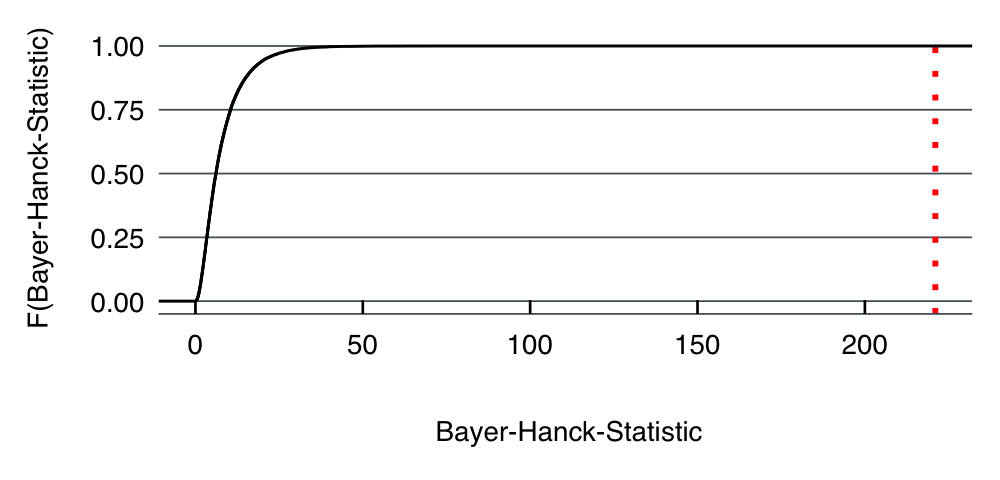
\includegraphics{plot_bh.png}
\caption{Cumulative Distribution Function under \(\mathcal{H}_0\)}
\end{figure}

\hypertarget{conclusion}{%
\section{Conclusion}\label{conclusion}}

The implementation of the R package \textbf{bayerhanck} has been
documented. It contains functions for two different versions of the
Bayer-Hanck Test for non cointegration, as well as functions for the
underlying cointegration tests. The former has been implemented in a
functional way, so that the functions \texttt{bayerhanck()} and
\texttt{bayerhanck\_1()} call the underlying test functions. Since the
underyling tests can be executed autonomously, the scope of application
is increased. The sub-functions certainly require more effort so the
tests can be applied to more versatile problems. This applies above all
to the tests of Banerjee and Boswijk, as we found no well working
implementation in R.

In the current version we also developed a further implementation with
the \texttt{bayerhanck\_1()} function. This function additionally
calculates the p-value of the test statistics based on the empirical
distribution stored in the function. For the aforementioned data set
with two regressors and approximately 26,000 observations, the function
needs about one second computation time. Further speed up of the
calculation might be desired, if one wants to work with bigger data. One
consideration might be to write the code directly in \texttt{C}, instead
of \texttt{R}, to save a step in the translation process.

Furthermore, two methods for the generic functions \texttt{summary()}
and \texttt{plot()} were defined Another implementation, which was not
covered in this documentation, is a user friendly application within a
shiny app. If it is published on a server, potential users might use the
functions of this package without using \texttt{R}themselves.

Of course, this package will be an object to further development. A
plausible advancement could be to increase the number of possible tests
and allow other combinations, than already implemented. For this, the
simulated distributions of the null distribution would have to be
stored. The power of each combination would have to be checked first.
However, this might lead to the problem, that users may tend to try out
different combinations, until they get their desired result.

\newpage
\renewcommand*{\mkbibnamefamily}[1]{\textbf{#1}}
\renewcommand*{\mkbibnamegiven}[1]{\textbf{#1}}
\renewcommand*{\mkbibnameprefix}[1]{\textbf{#1}}
\renewcommand*{\mkbibnamesuffix}[1]{\textbf{#1}}
\printbibliography[title=References]

\newpage
\textbf{Eidesstattliche Versicherung}

\bigskip

Ich versichere an Eides statt durch meine Unterschrift, dass ich die vorstehende Arbeit selbständig und ohne fremde Hilfe angefertigt und alle Stellen, die ich wörtlich oder annähernd wörtlich aus Veröffentlichungen entnommen habe, als solche kenntlich gemacht habe, mich auch keiner anderen als der angegebenen Literatur oder sonstiger Hilfsmittel bedient habe. Die Arbeit hat in dieser oder ähnlicher Form noch keiner anderen Prüfungsbehörde vorgelegen.

\vspace{1cm}
\rule{0pt}{2\baselineskip} %
\par\noindent\makebox[2.25in]{\indent Essen, den \hrulefill} \hfill\makebox[2.25in]{\hrulefill}%
\par\noindent\makebox[2.25in][l]{} \hfill\makebox[2.25in][c]{Name}%


\end{document}
